\documentclass[a4paper,12pt]{article}
\usepackage{graphicx}
\usepackage{amsmath}
\usepackage{array}
\usepackage{fancyhdr}
\usepackage{geometry}
\usepackage{titlesec}
\usepackage{tikz}
\usepackage{karnaugh-map}
\usetikzlibrary{circuits.logic.US, positioning}
\geometry{margin=1in}
\pagestyle{fancy}
\fancyhf{}
\rhead{EE24BTECH11012 - EE24BTECH11019}
\lhead{Experiment - 8}
\cfoot{\thepage}
\titleformat{\section}{\large\bfseries}{\thesection}{1em}{}

\begin{document}

\bibliographystyle{IEEEtran}
\vspace{3cm}

\title{EE1200 - ELECTRIC CIRCUITS LAB \\ \textbf{Experiment-8} }
\author{EE24BTECH11012 - Bhavanisankar G S \\ EE24BTECH11019 - Dwarak A}
% \maketitle
% \newpage
% \bigskip
\begin{center}
    
\includegraphics[width=0.5\textwidth]{IITH.png} \\ % Replace with your logo file
    \vspace{1cm} % Adjust spacing as needed
    \LARGE
    \end{center}
{\let\newpage\relax\maketitle}

\newpage
\tableofcontents
\newpage

\section{Objective}
The objective of this project is to design and implement a digital counter that keeps track of the number of people in a mess facility. The counter increments when a person enters and decrements when a person exits. The circuit should be built using basic logic gate ICs and JK flip-flops in a synchronous configuration, ensuring accurate, reliable, and glitch-free operation.

\section{Components Used}
\begin{itemize}
    \item AND, OR, NOT Gates (IC 7411, 7432, 7404)
    \item JK Flip-Flops (IC 7476)
    \item Seven Segment Display (Common Cathode)
    \item BCD to 7-Segment Decoder (IC 7447)
    \item Push Buttons (for simulating entry and exit)
    \item Resistors (1k$\Omega$, 10k$\Omega$)
    \item Breadboard, Connecting Wires
    \item 5V Power Supply ( from Arduino UNO )
\end{itemize}

\section{Theory}

\subsection{Synchronous Counters}
Synchronous counters use a common clock signal for all flip-flops, resulting in more predictable and synchronized state transitions compared to asynchronous counters. Each flip-flop changes state based on the inputs and the common clock edge.

\subsection{JK Flip-Flops}
JK Flip-Flops are versatile and can function as T flip-flops or D flip-flops based on how inputs are connected. In counters, they toggle when both J and K are high. The toggling condition is crucial for building up/down counters.

\subsection{Logic Gate ICs}
\begin{itemize}
    \item \textbf{7411 (AND gate)} – Provides logical AND operations.
    \item \textbf{7432 (OR gate)} – Provides logical OR operations.
    \item \textbf{7404 (NOT gate)} – Provides logical inversion.
\end{itemize}
These gates are used to generate control signals for counting and ensure that entry and exit signals do not conflict.

\subsection{Debouncing and Input Conditioning}
Mechanical buttons often produce bouncing effects, resulting in multiple transitions. This can be filtered using SR latches or simple RC debouncing circuits. For the purpose of this experiment, rapid pressing is avoided and basic logic gates are used to control invalid transitions.

\subsection{Block Diagram}
\begin{center}
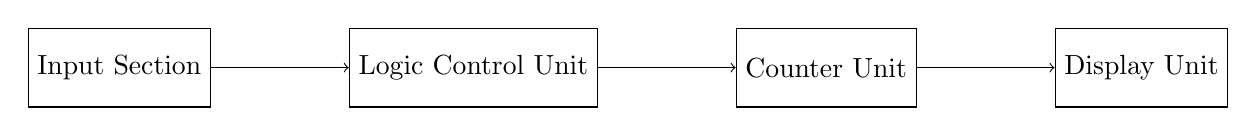
\begin{tikzpicture}[node distance=1.25cm and 1.75cm, every node/.style={draw, minimum height=1cm, minimum width=2cm}]
  \node (input) {Input Section};
  \node (logic) [right=of input] {Logic Control Unit};
  \node (counter) [right=of logic] {Counter Unit};
  \node (display) [right=of counter] {Display Unit};
  \draw[->] (input) -- (logic);
  \draw[->] (logic) -- (counter);
  \draw[->] (counter) -- (display);
\end{tikzpicture}

\textit{ Functional Block Diagram of the Mess Counter}
\end{center}

\subsection{Logic Control Circuit}
\begin{center}
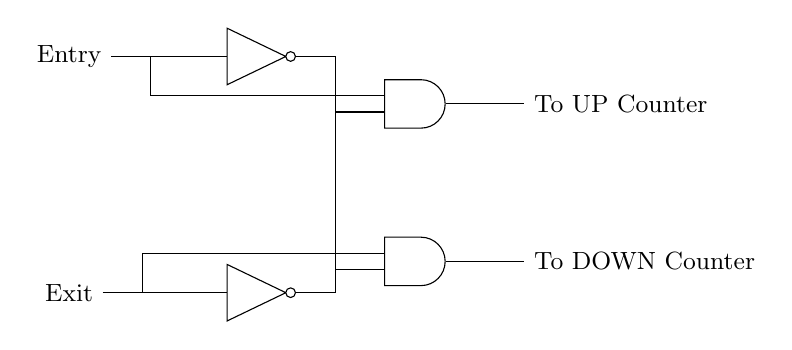
\begin{tikzpicture}[circuit logic US, every node/.style={font=\small}, scale=1, transform shape]

  % Entry and Exit labels
  \node at (0,3) (entry) {Entry};
  \node at (0,0) (exit) {Exit};

  % NOT gate for Exit (used in UP logic)
  \node[not gate, draw, anchor=input] (not1) at (2,0) {};
  \draw (exit.east) -- (not1.input);

  % AND gate for UP logic
  \node[and gate, draw, logic gate inputs=nn, anchor=input 1] (and1) at (4,2.5) {};
  \draw (entry.east) -- ++(0.5,0) |- (and1.input 1);
  \draw (not1.output) -- ++(0.5,0) |- (and1.input 2);
  \draw (and1.output) -- ++(1,0) node[right] {To UP Counter};

  % NOT gate for Entry (used in DOWN logic)
  \node[not gate, draw, anchor=input] (not2) at (2,3) {};
  \draw (entry.east) -- (not2.input);

  % AND gate for DOWN logic
  \node[and gate, draw, logic gate inputs=nn, anchor=input 1] (and2) at (4,0.5) {};
  \draw (exit.east) -- ++(0.5,0) |- (and2.input 1);
  \draw (not2.output) -- ++(0.5,0) |- (and2.input 2);
  \draw (and2.output) -- ++(1,0) node[right] {To DOWN Counter};

\end{tikzpicture}

\textit{Logic Gate Circuit Ensuring Mutual Exclusion of Entry and Exit}
\end{center}

\subsection{Truth Table and Logic Expressions}
\begin{table}[h!]
\centering
\begin{tabular}{|c|c|c|c|}
\hline
\textbf{Entry (E)} & \textbf{Exit (X)} & \textbf{UP} & \textbf{DOWN} \\
\hline
0 & 0 & 0 & 0 \\
1 & 0 & 1 & 0 \\
0 & 1 & 0 & 1 \\
1 & 1 & 0 & 0 \\
\hline
\end{tabular}
\caption{Truth Table for Logic Control}
\end{table}

\textbf{Raw Logic Expressions:}
\begin{itemize}
  \item UP = E \(\cdot\) \(\overline{X}\)
  \item DOWN = X \(\cdot\) \(\overline{E}\)
\end{itemize}

\subsection{Counter Circuit}
\begin{center}

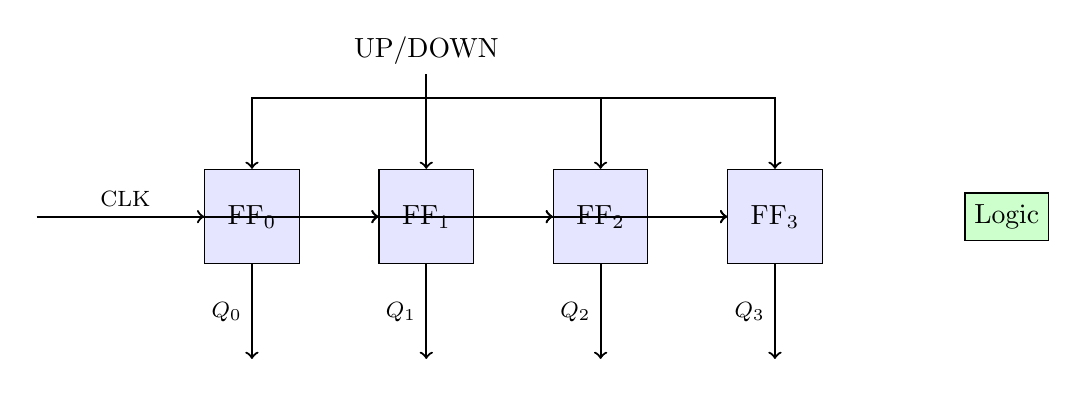
\begin{tikzpicture}[
  flipflop/.style={draw, minimum width=1.2cm, minimum height=1.2cm, fill=blue!10},
  signal/.style={->, thick},
  label/.style={font=\footnotesize},
  node distance=1.6cm and 1cm
]

% Flip-Flops
\node[flipflop] (ff0) {FF$_0$};
\node[flipflop, right=of ff0] (ff1) {FF$_1$};
\node[flipflop, right=of ff1] (ff2) {FF$_2$};
\node[flipflop, right=of ff2] (ff3) {FF$_3$};

% Clock input
\node[left=2cm of ff0] (clk) {};
\draw[signal] (clk) -- node[above, label] {CLK} (ff0.west);

% Clock distribution
\draw[signal] (clk) |- (ff1.west);
\draw[signal] (clk) |- (ff2.west);
\draw[signal] (clk) |- (ff3.west);

% Q outputs
\foreach \i/\ff in {0/ff0,1/ff1,2/ff2,3/ff3} {
  \node[below=1.2cm of \ff] (q\i) {};
  \draw[signal] (\ff.south) -- node[label, left] {$Q_\i$} (q\i);
}

% Up/Down control
\node[above=1.2cm of ff1] (ud) {UP/DOWN};
\draw[signal] (ud) -- ++(0,-0.6) -| (ff0.north);
\draw[signal] (ud) -- ++(0,-0.6) -| (ff1.north);
\draw[signal] (ud) -- ++(0,-0.6) -| (ff2.north);
\draw[signal] (ud) -- ++(0,-0.6) -| (ff3.north);

% AND/OR gates or control logic hint
\node[draw, fill=green!20, minimum width=1cm, minimum height=0.6cm, right=1.8cm of ff3] (control) {Logic};
\draw[signal] (ff0.east) -- (ff1.west);
\draw[signal] (ff1.east) -- (ff2.west);
\draw[signal] (ff2.east) -- (ff3.west);

\end{tikzpicture}

\textit{(Figure: Synchronous 4-bit Up/Down Counter using JK Flip-Flops)}
\end{center}

\subsection{Display Decoder Circuit}
\begin{center}
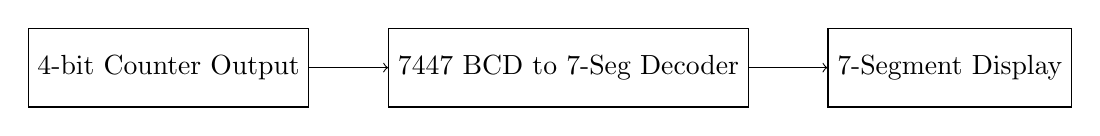
\begin{tikzpicture}[every node/.style={draw, minimum height=1cm, minimum width=2.5cm}]
  \node (bcd) {4-bit Counter Output};
  \node (decoder) [right=of bcd] {7447 BCD to 7-Seg Decoder};
  \node (display) [right=of decoder] {7-Segment Display};
  \draw[->] (bcd) -- (decoder);
  \draw[->] (decoder) -- (display);
\end{tikzpicture}

\textit{(Figure: Interfacing Counter Output with Display)}
\end{center}

\subsection{Circuit Description}
The circuit is composed of the following major parts:
\begin{enumerate}
    \item \textbf{Input Section:} Two push buttons are used—one for entry and one for exit. These generate control signals for counting.
    \item \textbf{Logic Control Unit:} Logic gates ensure that only one action (increment or decrement) occurs at a time. If both buttons are pressed simultaneously, no change is registered.
    \item \textbf{Counter Unit:} A 4-bit synchronous up-down counter is built using JK Flip-Flops. Entry signals cause an up count, and exit signals cause a down count.
    \item \textbf{Display Unit:} The output of the counter is fed into a 7447 BCD to 7-segment decoder which drives a common cathode display.
\end{enumerate}

\section{Truth Table}
\begin{table}[h]
\centering
\begin{tabular}{|c|c|c|c|c|}
    \hline
    \textbf{Entry} & \textbf{Exit} & \textbf{Action} & \textbf{Count (Before)} & \textbf{Count (After)} \\
    \hline
    0 & 0 & No Change & N & N \\
    1 & 0 & Increment & N & N+1 \\
    0 & 1 & Decrement & N & N-1 \\
    1 & 1 & Invalid (No Change) & N & N \\
    \hline
\end{tabular}
\caption{Truth Table for Entry/Exit Logic}
\end{table}

\subsection{Timing Diagram}
\begin{figure}[h]
\centering
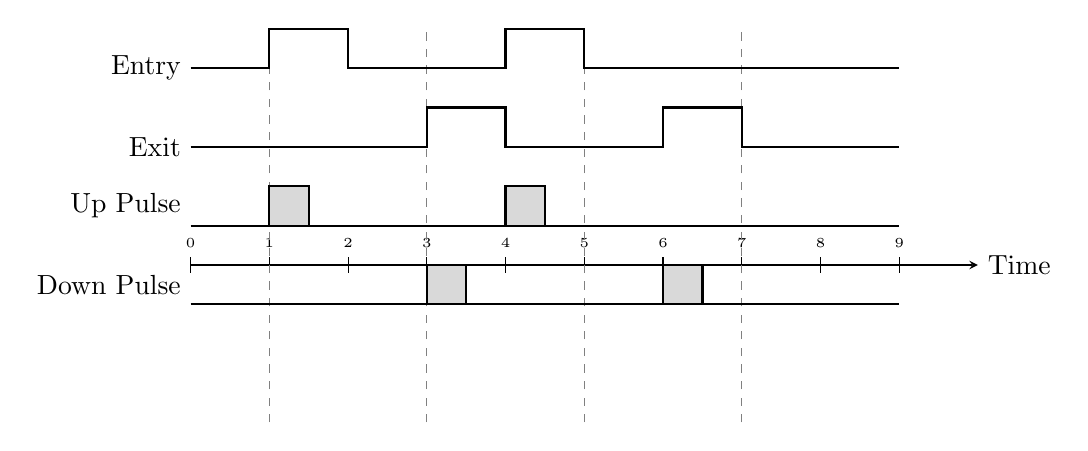
\begin{tikzpicture}[>=stealth]
    % Define parameters
    \def\clkwidth{0.5}
    \def\high{1}
    \def\low{0}
    \def\pulseheight{0.5}
    
    % Time axis
    \draw[->] (0,0) -- (10,0) node[right] {Time};
    \foreach \x in {0,1,...,9} {
        \draw (\x,-0.1) -- (\x,0.1) node[above, font=\tiny] {\x};
    }
    
    % Vertical lines for alignment
    \foreach \x in {1,3,5,7} {
        \draw[dashed, gray] (\x,-2) -- (\x,3);
    }
    
    % Entry signal
    \draw[thick] (0,2.5) -- (1,2.5) -- (1,3) -- (2,3) -- (2,2.5) -- (4,2.5) -- (4,3) -- (5,3) -- (5,2.5) -- (9,2.5);
    \node[left] at (0,2.5) {Entry};
    
    % Exit signal
    \draw[thick] (0,1.5) -- (3,1.5) -- (3,2) -- (4,2) -- (4,1.5) -- (6,1.5) -- (6,2) -- (7,2) -- (7,1.5) -- (9,1.5);
    \node[left] at (0,1.5) {Exit};
    
    % Up pulse
    \draw[thick] (0,0.5) -- (1,0.5);
    \draw[thick, fill=gray!30] (1,0.5) rectangle (1.5,1);
    \draw[thick] (1.5,0.5) -- (4,0.5);
    \draw[thick, fill=gray!30] (4,0.5) rectangle (4.5,1);
    \draw[thick] (4.5,0.5) -- (9,0.5);
    \node[left] at (0,0.75) {Up Pulse};
    
    % Down pulse
    \draw[thick] (0,-0.5) -- (3,-0.5);
    \draw[thick, fill=gray!30] (3,-0.5) rectangle (3.5,0);
    \draw[thick] (3.5,-0.5) -- (6,-0.5);
    \draw[thick, fill=gray!30] (6,-0.5) rectangle (6.5,0);
    \draw[thick] (6.5,-0.5) -- (9,-0.5);
    \node[left] at (0,-0.25) {Down Pulse};
\end{tikzpicture}
\caption{Timing diagram showing Entry, Exit, and corresponding counter pulses}
\end{figure}

\subsection{Derivation of Logic}

Below are the state tables and Karnaugh map derivations for both the up and down counter modes.

\subsection*{State Tables}

\textbf{Up Counter State Table:}
\begin{table}[h]
\centering
\begin{tabular}{|c|c|c|c||c|c|c|c||c|c|c|c|}
\hline
\multicolumn{4}{|c||}{Present State} & \multicolumn{4}{c||}{T Flip-Flops} & \multicolumn{4}{c|}{Next State} \\
\hline
\(Q_3\) & \(Q_2\) & \(Q_1\) & \(Q_0\) & \(T_3\) & \(T_2\) & \(T_1\) & \(T_0\) & \(Q_3\) & \(Q_2\) & \(Q_1\) & \(Q_0\) \\
\hline
0 & 0 & 0 & 0 & 0 & 0 & 0 & 1 & 0 & 0 & 0 & 1 \\
\hline
0 & 0 & 0 & 1 & 0 & 0 & 1 & 1 & 0 & 0 & 1 & 0 \\
\hline
0 & 0 & 1 & 0 & 0 & 0 & 0 & 1 & 0 & 0 & 1 & 1 \\
\hline
0 & 0 & 1 & 1 & 0 & 1 & 1 & 1 & 0 & 1 & 0 & 0 \\
\hline
0 & 1 & 0 & 0 & 0 & 0 & 0 & 1 & 0 & 1 & 0 & 1 \\
\hline
0 & 1 & 0 & 1 & 0 & 0 & 1 & 1 & 0 & 1 & 1 & 0 \\
\hline
0 & 1 & 1 & 0 & 0 & 0 & 0 & 1 & 0 & 1 & 1 & 1 \\
\hline
0 & 1 & 1 & 1 & 1 & 1 & 1 & 1 & 1 & 0 & 0 & 0 \\
\hline
1 & 0 & 0 & 0 & 0 & 0 & 0 & 1 & 1 & 0 & 0 & 1 \\
\hline
1 & 0 & 0 & 1 & 1 & 0 & 0 & 1 & 0 & 0 & 0 & 0 \\
\hline
1 & 0 & 1 & 0 & X & X & X & X & X & X & X & X \\
\hline
1 & 0 & 1 & 1 & X & X & X & X & X & X & X & X \\
\hline
1 & 1 & 0 & 0 & X & X & X & X & X & X & X & X \\
\hline
1 & 1 & 0 & 1 & X & X & X & X & X & X & X & X \\
\hline
1 & 1 & 1 & 0 & X & X & X & X & X & X & X & X \\
\hline
1 & 1 & 1 & 1 & X & X & X & X & X & X & X & X \\
\hline
\end{tabular}
\caption{State table for the single-digit BCD Up-counter. (X denotes don't-care conditions.)}
\end{table}

\vspace{0.5cm}
\textbf{Down Counter State Table:}
\begin{table}[h]
\centering
\begin{tabular}{|c|c|c|c||c|c|c|c||c|c|c|c|}
\hline
\multicolumn{4}{|c||}{Present State} & \multicolumn{4}{c||}{T Flip-Flops} & \multicolumn{4}{c|}{Next State} \\
\hline
\(Q_3\) & \(Q_2\) & \(Q_1\) & \(Q_0\) & \(T_3\) & \(T_2\) & \(T_1\) & \(T_0\) & \(Q_3\) & \(Q_2\) & \(Q_1\) & \(Q_0\) \\
\hline
0 & 0 & 0 & 0 & 1 & 0 & 0 & 1 & 1 & 0 & 0 & 1 \\
\hline
0 & 0 & 0 & 1 & 0 & 0 & 0 & 1 & 0 & 0 & 0 & 0 \\
\hline
0 & 0 & 1 & 0 & 0 & 0 & 1 & 1 & 0 & 0 & 0 & 1 \\
\hline
0 & 0 & 1 & 1 & 0 & 0 & 0 & 1 & 0 & 0 & 1 & 0 \\
\hline
0 & 1 & 0 & 0 & 0 & 1 & 1 & 1 & 0 & 0 & 1 & 1 \\
\hline
0 & 1 & 0 & 1 & 0 & 0 & 0 & 1 & 0 & 1 & 0 & 0 \\
\hline
0 & 1 & 1 & 0 & 0 & 0 & 1 & 1 & 0 & 1 & 0 & 1 \\
\hline
0 & 1 & 1 & 1 & 0 & 0 & 0 & 1 & 0 & 1 & 1 & 0 \\
\hline
1 & 0 & 0 & 0 & 1 & 1 & 1 & 1 & 0 & 1 & 1 & 1 \\
\hline
1 & 0 & 0 & 1 & 0 & 0 & 0 & 1 & 1 & 0 & 0 & 0 \\
\hline
1 & 0 & 1 & 0 & X & X & X & X & X & X & X & X \\
\hline
1 & 0 & 1 & 1 & X & X & X & X & X & X & X & X \\
\hline
1 & 1 & 0 & 0 & X & X & X & X & X & X & X & X \\
\hline
1 & 1 & 0 & 1 & X & X & X & X & X & X & X & X \\
\hline
1 & 1 & 1 & 0 & X & X & X & X & X & X & X & X \\
\hline
1 & 1 & 1 & 1 & X & X & X & X & X & X & X & X \\
\hline
\end{tabular}
\caption{State table for the single-digit BCD Down-counter. (X denotes don't-care conditions.)}
\end{table}

\newpage
\subsection*{Karnaugh Maps for T Flip-Flops}

\subsubsection*{Up Counter T Flip-Flops}
\textbf{For \(T_0\):}\\
Since \(T_0 = 1\) for all cases, no Karnaugh map is required.

\vspace{0.5cm}
\textbf{For \(T_1\):}
\begin{center}
\begin{karnaugh-map}[4][4][1][$Q_1Q_0$][$Q_3Q_2$]
\manualterms{0,1,0,1,0,1,0,1,0,0,X,X,X,X,X,X}
\end{karnaugh-map}
\end{center}
Thus, 
\[
T_1 = \overline{Q_3}\,Q_0.
\]

\vspace{0.3cm}
\textbf{For \(T_2\):}
\begin{center}
\begin{karnaugh-map}[4][4][1][$Q_1Q_0$][$Q_3Q_2$]
\manualterms{0,0,0,1,0,0,0,1,0,0,X,X,X,X,X,X}
\end{karnaugh-map}
\end{center}
Thus, 
\[
T_2 = Q_1\,Q_0.
\]

\vspace{0.5cm}
\textbf{For \(T_3\):}
\begin{center}
\begin{karnaugh-map}[4][4][1][$Q_1Q_0$][$Q_3Q_2$]
\manualterms{0,0,0,0,0,0,0,1,0,1,X,X,X,X,X,X}
\end{karnaugh-map}
\end{center}
Thus, 
\[
T_3 = Q_2\,Q_1\,Q_0 + Q_3\,Q_0.
\]
\[
T_3 = Q_2\,T_2 + Q_3\,Q_0 
\]


\subsubsection*{Down Counter T Flip-Flops}
\textbf{For \(T_0\):}\\  
Again, \(T_0 = 1\) for all cases.

\vspace{0.5cm}
\textbf{For \(T_1\):}
\begin{center}
\begin{karnaugh-map}[4][4][1][$Q_1Q_0$][$Q_3Q_2$]
\manualterms{0,0,1,0,1,0,1,0,1,0,X,X,X,X,X,X}
\end{karnaugh-map}
\end{center}
Thus,
\[
T_1 = Q_1\,\overline{Q_0} + Q_2\,\overline{Q_1}\,\overline{Q_0} + Q_3\,\overline{Q_1}\,\overline{Q_0}.
\]
\[
T_1 = Q_1\,\overline{Q_0} + T_2
\]

\vspace{0.5cm}
\textbf{For \(T_2\):}
\begin{center}
\begin{karnaugh-map}[4][4][1][$Q_1Q_0$][$Q_3Q_2$]
\manualterms{0,0,0,0,1,0,0,0,1,0,X,X,X,X,X,X}
\end{karnaugh-map}
\end{center}
Thus,
\[
T_2 = Q_2\,\overline{Q_1}\,\overline{Q_0} + Q_3\,\overline{Q_1}\,\overline{Q_0}.
\]

\vspace{0.5cm}
\textbf{For \(T_3\):}
\begin{center}
\begin{karnaugh-map}[4][4][1][$Q_1Q_0$][$Q_3Q_2$]
\manualterms{1,0,0,0,0,0,0,0,1,0,X,X,X,X,X,X}
\end{karnaugh-map}
\end{center}
Thus,
\[
T_3 = \overline{Q_2}\,\overline{Q_1}\,\overline{Q_0}.
\]

\begin{figure}[h]
    \centering
    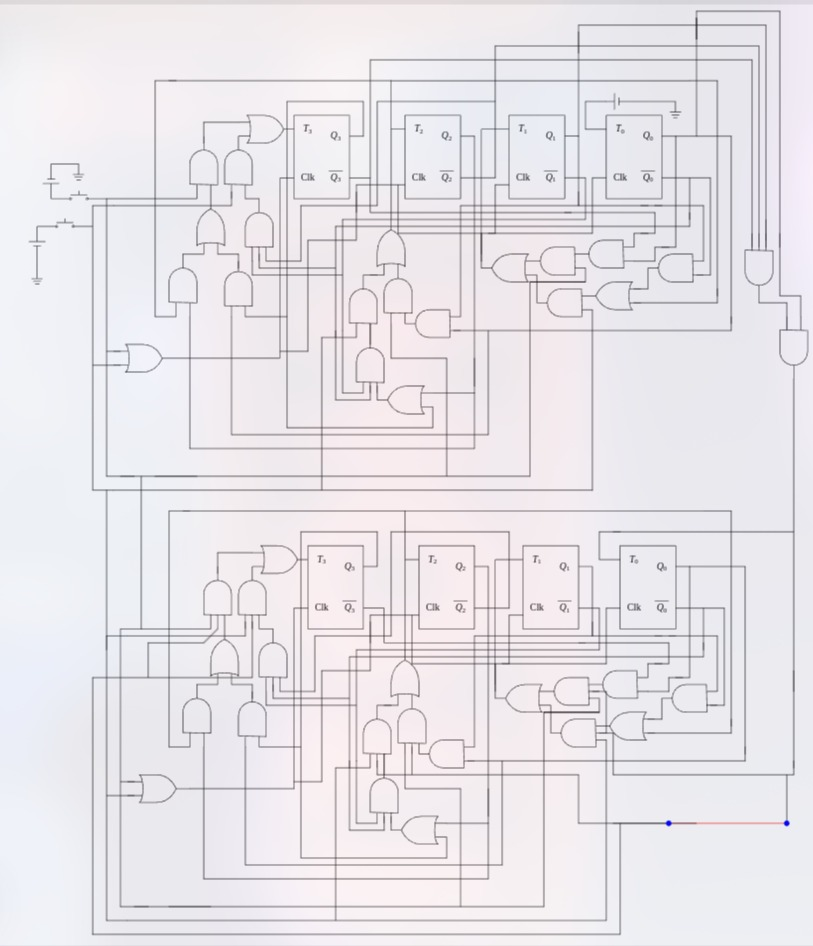
\includegraphics[width=0.7\textwidth]{1.jpg} % no file extension needed if it's a .pdf, .png or .jpg
    \caption{Complete circuit}
    \label{fig:example}
\end{figure}

\section{Procedure}
\subsection{Circuit Connections}
The detailed connections between components are as follows:

\begin{itemize}
    \item \textbf{Input Circuit:}
    \begin{itemize}
        \item Entry push button connected to +5V with a 10k$\Omega$ pull-down resistor
        \item Exit push button connected to +5V with a 10k$\Omega$ pull-down resistor
    \end{itemize}
    
    \item \textbf{Logic Control Unit:}
    \begin{itemize}
        \item IC 7411 (AND gate): 
        \begin{itemize}
            \item Pin 1 \& 2 (inputs) connected to Entry button and inverted Exit signal
            \item Pin 3 (output) gives Up count signal
            \item Pin 4 \& 5 (inputs) connected to Exit button and inverted Entry signal
            \item Pin 6 (output) gives Down count signal
            \item The other input in both the cases is connected to $V_{cc}$
        \end{itemize}
        \item IC 7404 (NOT gate):
        \begin{itemize}
            \item Pin 1 (input) connected to Exit button
            \item Pin 2 (output) connected to AND gate for Up count
            \item Pin 3 (input) connected to Entry button
            \item Pin 4 (output) connected to AND gate for Down count
        \end{itemize}
    \end{itemize}
    
    \item \textbf{JK Flip-Flop Counter:}
    \begin{itemize}
        \item For each 7476 JK Flip-Flop:
        \begin{itemize}
            \item J and K inputs connected to control logic based on up/down counting
            \item Clock inputs connected to common clock signal
            \item Q outputs connected to next flip-flop's control logic
            \item $\overline{Q}$ outputs used for control logic
        \end{itemize}
        \item For up counting: Each flip-flop toggles when all previous flip-flops are at logic 1
        \item For down counting: Each flip-flop toggles when all previous flip-flops are at logic 0
    \end{itemize}
    
    \item \textbf{Display Unit:}
    \begin{itemize}
        \item IC 7447 BCD to 7-segment decoder:
        \begin{itemize}
            \item Pins 7, 1, 2, 6 (A, B, C, D inputs) connected to Q0, Q1, Q2, Q3 of counter
            \item Pins 13, 12, 11, 10, 9, 15, 14 (a-g outputs) connected to 7-segment display
        \end{itemize}
        \item 7-segment display:
        \begin{itemize}
            \item Common cathode connected to ground through a 220$\Omega$ resistor
            \item Segments connected to decoder outputs through 330$\Omega$ current-limiting resistors
        \end{itemize}
    \end{itemize}
\end{itemize}

\begin{figure}[h]
\centering
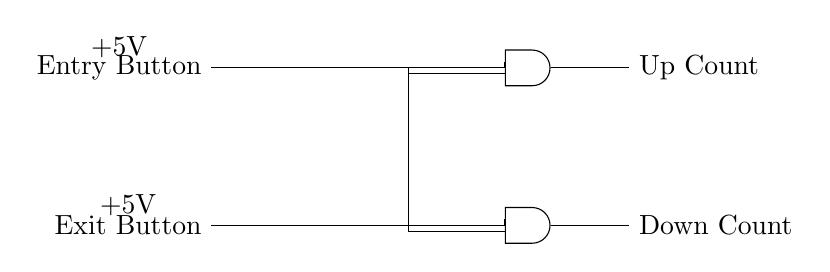
\begin{tikzpicture}[circuit logic US, node distance=2cm]
    % Input buttons
    \node[left] (entry) at (0,2) {Entry Button};
    \node[left] (exit) at (0,0) {Exit Button};
    
    % NOT gates
    \coordinate (entrypoint) at (1,2);
    \coordinate (exitpoint) at (1,0);
    
    \draw (entry) -- (entrypoint);
    \draw (exit) -- (exitpoint);
    
    \draw (exitpoint) -- ++(1,0) node[not gate US, anchor=input] (not1) {};
    \draw (entrypoint) -- ++(1,0) node[not gate US, anchor=input] (not2) {};
    
    % AND gates
    \node[and gate US, draw, logic gate inputs=nn] (upand) at (4,2) {};
    \node[and gate US, draw, logic gate inputs=nn] (downand) at (4,0) {};
    
    \draw (entrypoint) -| (upand.input 1);
    \draw (not1.output) |- (upand.input 2);
    
    \draw (exitpoint) -| (downand.input 1);
    \draw (not2.output) |- (downand.input 2);
    
    % Control signals
    \draw (upand.output) -- ++(1,0) node[right] {Up Count};
    \draw (downand.output) -- ++(1,0) node[right] {Down Count};
    
    % Draw labels
    \node[above] at (entry) {+5V};
    \node[above] at (exit) {+5V};
\end{tikzpicture}
\caption{Detailed Logic Control Circuit Connections}
\end{figure}


\section{Observations and Results}
\begin{itemize}
    \item Initial state is 0000 (0 count).
    \item Each press of the entry button increases count by 1.
    \item Each press of the exit button decreases count by 1.
    \item Simultaneous press of both buttons does not affect the count.
    \item Display reflects the correct count in real-time.
    \item It is observed that the counter resets the value to 0 and decrementing from 0 results in 99. This is a drawback to this connection.
\end{itemize}

\begin{figure}[h]
    \centering
    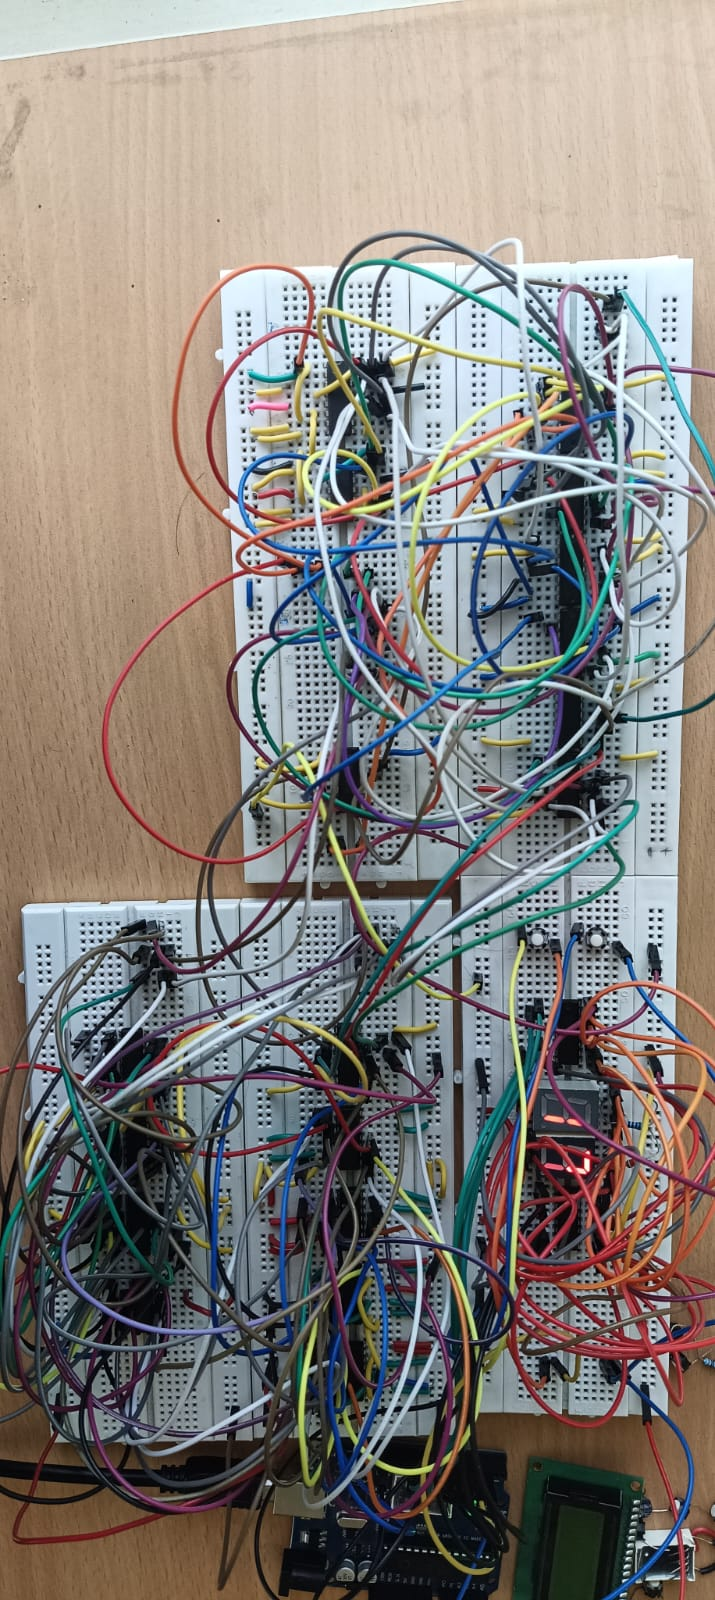
\includegraphics[width=0.7\textwidth]{2.jpg} % no file extension needed if it's a .pdf, .png or .jpg
    \caption{Figure}
    \label{fig:example}
\end{figure}


\end{document}
